% CHAPTER - State of the Art ---------------------

% This section lists the current knowledge in the field of your research question

% Start with some more general aspects and go deeper into the specific research field of your thesis

% Ends with description of knowledge closely related to thesis work
 
% \cite{} vs. \citep{} (citeparentesis)

\chapter{Estado da Arte}
    
    A decomposição de sistemas em módulos é um tópico que começou a ser sistematizado e debatido por \cite{parnas72_decomposing_systems} muito antes da massificação dos sistemas de \textit{software}. Neste seu trabalho, Parnas, pretende demonstrar que a eficiência da modularização de um sistema depende do critério utilizado, não sendo apenas a fragmentação em pequenos módulos o trajeto para o sucesso, mas sim a forma como é feita a escolha do critério de segregação. 
    
    % refazer este parágrafo, não se pode dizer que o encapsulamento é melhor e depois não seguir esse método. Ou se remove, ou se descreve que existem os dois métodos e nós fomos por um deles 
    % [ESTOU A CONTRARIARME NESTA FRASE]    Desta forma, recorre à apresentação e a análise de dois critérios distintos para um caso de estudo: o primeiro focado no fluxo do algoritmo e o segundo na ocultação de informação inerente a cada módulo. Realiza de seguida, uma análise comparativa relativa a propriedades de esforço de desenvolvimento, flexibilidade e compreensibilidade. A análise permite concluir que uma decomposição baseada na ocultação de informação é superior dada a forma como as mudanças são mais localizadas e não obrigam a alterações de \textit{design} que abranjam múltiplos módulos do sistema \cite{parnas72_decomposing_systems}. 
   
    A relevância da decomposição funcional de sistemas inicialmente referida por Parnas, reforçou-se pela necessidade na atualidade em distribuir sistemas complexos por infraestruturas de rede como \textit{web services} e objetos remotos resultante dos esforços em lidar com sistemas de maior dimensão e complexidade \citep{kamimura18_city_analogy}. 
    
    Os principais desafios desta decomposição passam pelo trabalho manual e tedioso acompanhado da dificuldade em identificar as unidades funcionais dada a necessidade de uma análise detalhada de várias dimensões da arquitetura de \textit{software}, estando muitas vezes a qualidade do resultado final fortemente ligada à experiência e o conhecimento do especialista que realiza a decomposição \citep{kamimura18_city_analogy, pahl16_ms_systematic_mapping}. 
    


\section{Migração manual de monólitos para micro-serviços}

   Nesta secção é realizada uma análise da bibliografia relativamente a processos de migração de arquiteturas monolíticas para micro-serviços realizados de forma manual, por especialistas, em projetos de escala industrial. Procura-se fazer uma identificação de conhecimento sobre que elementos do processo de transição podem ser identificados e sistematizados com o objetivo de recolher informação útil à automatização do processo.
    
    Com o crescer da popularidade do uso de arquiteturas de micro-serviços como uma alternativa a alguns dos problemas inerentes às arquiteturas monolíticas também assim cresceu a necessidade de formalização dos seus métodos. Muitos arquitetos de soluções de \textit{software} vêem como uma vantagem a transição da sua aplicação \textit{legacy} para micro-serviços com o objetivo de melhorar e tornar mais eficiente o processo de desenvolvimento de \textit{software}. 
    
    Esta migração é um processo complexo, muito dependente do domínio do \textit{software} que poderá exigir várias iterações até se poder dar por concluída \citep{dehghani18_break_monolith_into_microservices}.
    
    % A escassa literatura que formalize este processo \citep{balalaie18_ms_migration_patterns} 
    
    
    Com o intuito de combater a vertente \textit{ad-hoc} realizada até ao momento no processo de migração, \cite{balalaie18_ms_migration_patterns} recolheram um conjunto de \textit{design patterns} identificados empiricamente pela análise de processos de migração de aplicações de calibre industrial. Neste trabalho procura-se fazer uma análise que englobe todo o processo de migração, desde a identificação da arquitetura atual e decomposição da respetiva em diferentes serviços, a processos inerentes ao \textit{DevOps} e à migração para a \textit{cloud} como o \textit{CI}, \textit{CD}, introdução de \textit{service discovery}, \textit{load balancing}, orquestração de \textit{containers}, \textit{etc}.
    
    Visto que um método rígido, do estilo \textit{one-size-fits-all} nunca seria funcional dado a elevada unicidade resultante de soluções complexas e específicas de determinado domínio, e variedade como os sistemas de \textit{software} são compostos, \cite{balalaie18_ms_migration_patterns} recorrem a uma abordagem designada por \textit{Situational Method Engineering (SME)} \citep{situational_method_engineering}. De uma forma concisa, um método pode ser projetado de acordo com a situação em específico \citep{balalaie18_ms_migration_patterns}.
    % unico 
    
    Do seu estudo empírico e aplicação do \textit{SME} resultou um repositório de 16 padrões, acompanhado de um plano de migração, Figura \ref{fig:plano_migracao_migroservicos} que procura ao longo do processo lidar com possíveis dependências situacionais entre as diversas etapas.
    
	\begin{figure}[h]
     	\begin{center}
     		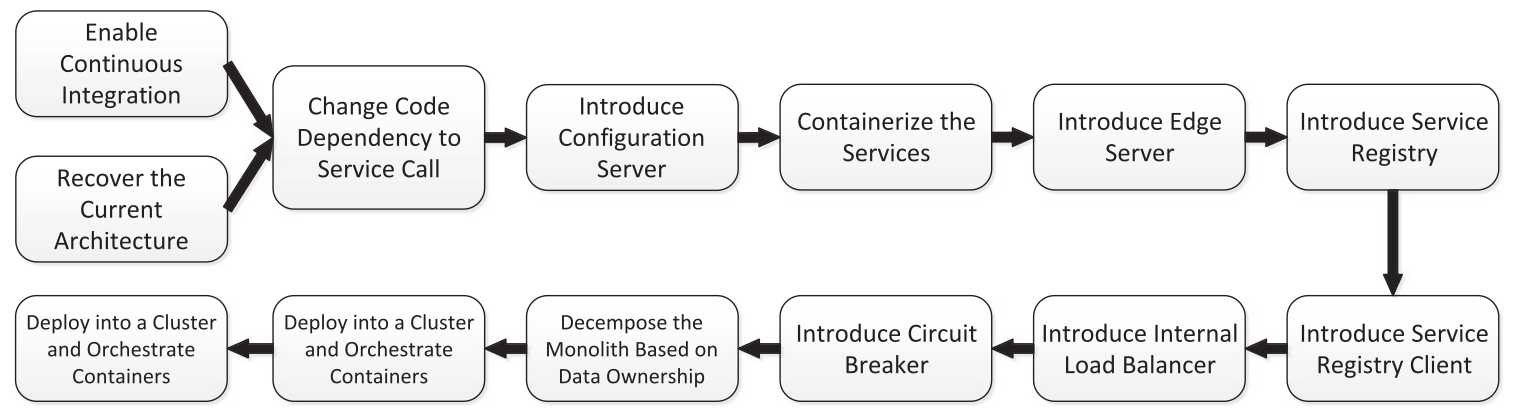
\includegraphics[width=\textwidth]{img/migration_plan.png}
     	\end{center}
     	\caption{Plano de migração proposto}
     	\label{fig:plano_migracao_migroservicos}
     	\floatfoot{Source: \cite{balalaie18_ms_migration_patterns}}
 	\end{figure}
    % TODO: adicionar source da imagem	
    % e ter o menor impacto possível nos utilizadores finais. o que realmente significa isto?
    
    No contacto com três empresas que realizaram a migração do seu monólito de grande escala, constataram que dos 16 padrões identificados, 85\% foram utilizados na migração para micro-serviços.
    
     % rever o que significa ao certo os utilizadores finais neste contexto?
    
    Com um objetivo semelhante de investigar e sistematizar o processo de migração, \cite{fritzsch19_migration_in_industry} realizaram um estudo qualitativo relativamente às intenções, estratégias e desafios no processo de migração de 14 sistemas de larga escala com períodos de migração expectáveis entre 1.5 e 3 anos) de diversos domínios (sistemas de transportes públicos, gestão de hotéis, retalho, etc.), recorrendo a entrevistas detalhadas de 16 profissionais experientes de 10 empresas diferentes. 
    
    Da análise realizada, concluem que a dificuldade em lidar com a manutenção dos sistemas e a necessidade de escalabilidade mais eficiente continuam a ser os factores cruciais a originar a transição para micro-serviços. Um dos principais desafios reportados no processo de migração tratou-se de como fazer a decomposição dos sistemas. Sete participantes apostaram numa decomposição funcional, descrita por \cite{fowler14_definition_microservices}, recorrendo quatro deles à utilização explicita de \textit{domain-driven design}. Os restantes participantes optaram por abordagens não sistematizadas \citep{fritzsch19_migration_in_industry}.
    
    De todos os participantes do estudo, nenhum considerou ou tinha consciência da utilização de técnicas de auxílio na decomposição dos seus sistemas (ex.: análise estática de código, análise de \textit{execution traces}) \cite{fritzsch19_migration_in_industry}. Seis dos participantes fizeram propostas de micro-serviços com anti-padrões (\textit{Wrong Cuts, Shared Persistency, Service Intimacy}, padrões identificados por \cite{taibi18_architectural_patterns}), resultantes de decomposições inapropriadas.
    
%    \todo{conclusão e transição}
    
    
    Apesar do massivo adaptar de arquiteturas de micro-serviços, há especialistas, como \cite{fowler15_monolith_first}, que defendem que um sistema de \textit{software} terá maior sucesso se for construído inicialmente segundo uma arquitetura monolítica e posteriormente migrado para micro-serviços assim que a complexidade comece a ganhar relevância. Desta forma, uma arquitetura inicial monolítica permite um melhor explorar da complexidade do sistema e os limites dos componentes \cite{fowler15_monolith_first}. 
    Há já elevada necessidade de formalizar esta migração, ideias como esta apresentadas por \textit{Fowler} manterão a relevância da contínua necessidade de investigação e formalização de métodos que tornem mais eficiente e eficaz a migração de arquiteturas monolíticas para micro-serviços.
    
    % REFERIDO NUM ARTIGO ACIMA(?): falta de aderência à literatura 
    
    % como deve ser feito
    % qual será o tamanho esperado
    % bounding context  
    
    É descrito de seguida o estado da arte das áreas de conhecimento mais promissoras à solução do problema em questão.

\section{Soluções de migração orientados ao código fonte}

    Dado que o objetivo final passará pela decomposição do código fonte de uma aplicação monolítica em vários micro-serviços, uma abordagem recorrendo ao código fonte será uma das abordagens mais evidentes, dado que permitirá trabalhar com granularidades finas e manipular livremente o código possibilitando a conjugação com outras áreas de estudo.

\subsection{Análise estática}

    A análise estática é muito utilizada nas áreas de testes de \textit{software} para identificação de \textit{bugs}, análise de complexidade do código, entre outros, esta técnica é também promissora nesta área dada a necessidade em trabalhar sobre o código fonte e realizar a sua manipulação.
    
    Com o intuito de uma abordagem estática, \cite{mazlami17} propõem no seu trabalho 3 estratégias formais de acoplamento posteriormente processadas segundo algoritmos de \textit{clustering}. As estratégias propostas baseiam-se na combinação do código fonte da aplicação monolítica e seus meta-dados, recolhidos do sistema de versões \textit{Git}. 
    
    Das estratégias de acoplamento propostas pelos autores, o acoplamento lógico, baseia-se na premissa que as alterações feitas num monólito são realizadas apenas a um módulo em específico, desta forma, analisa-se o histórico de alterações tendo em conta que as classes que se alteram juntas também deverão estar juntas num micro-serviço. O acoplamento semântico, baseia-se em agrupar classes que têm código sobre as mesmas coisas, ou seja, calculando a similaridade de termos de domínio entre duas classes poderá obter-se uma medida para identificar quão semanticamente próximas são as classes. Por fim, acoplamento por contribuição, baseado na lei de \cite{conwayslaw}, que indica que a estrutura de \textit{software} representa a estrutura da organização, e como tal, módulos específicos que recebem alterações de um conjunto único de elementos da equipa devem manter-se no mesmo micro-serviço. Cada uma das técnicas de acoplamento é utilizada no processo inicial de extração, sendo posteriormente construído um grafo de dependências que será utilizado para aplicação de algoritmos de \textit{clustering}.
    
    % TODO : transição e mais contexto??
    O \textit{clustering} realizado opera apenas sobre a \textit{minimum spanning tree}\footnote{\textit{Subset} dos vértices de um grafo não direcionado no qual todos os vértices são conectados pelo menor peso possível total das arestas, sem a ocorrência de ciclos.} para garantir que cada remoção de um arco resulta num aumento no número de componentes conectados. No entanto, essa operação introduz a desvantagem de deixar de fora algumas das conexões inicialmente obtidas pelo método de acoplamento limitando a proposta de serviços \citep{mazlami17}. Outro fator limitante deste trabalho expressa-se pelo uso de classes como a unidade atómica de identificação e extração dos micro-serviços, tornando impossível a segregação de componentes de uma classe para vários micro-serviços.
    
    % dar contexto sobre o endpoint na secção de contexto
    \cite{kamimura18_city_analogy} recorrem também a técnicas de \textit{clustering} para realizar as suas propostas de micro-serviços. A extração das classes é iniciada pela identificação dos \textit{endpoints} da API da aplicação em questão, recorrendo a anotações de \textit{frameworks} específicas (ex.: \textit{@Controller} em \textit{Spring}), que identificam os \textit{endpoints} expostos em APIs REST. Para extração de restante conhecimento, recorre-se também a anotações como o \textit{@Entity} e \textit{@Table} para identificar as classes responsáveis por definir a persistência e tratamento dos dados. O método de \textit{clustering} referido neste trabalho tem como um dos principais objetivos lidar com módulos omnipresentes, ou seja, módulos com um elevado número de relações com outros módulos e presentes numa elevada quantidade de módulos. Proposto por \cite{kobayashi12_feature_gathering_software_clustering}, esta estratégia pretende abordar esse problema por enfraquecer a importância atribuída a módulos com essa particularidade facilitando o processo de \textit{clustering} dos componentes \citep{kobayasi13_sarf}. 
    
%    \todo{Dar mais contexto sobre o trabalho}
    
    Neste trabalho de \cite{kamimura18_city_analogy} apenas se realiza a proposta de micro-serviços não existindo qualquer extração ou \textit{refactor} do código submetido a avaliação.
    
    % NOTAS SOBRE ARTIGO ACIMA: 
    %  - Não fazem o refactor, só fazem a proposta de extração
    %  - Necessita que as classes contendo os endpoints sejam indicadas inicialmente
    
    
    


\subsection{Análise dinâmica}
    
    As técnicas de análise dinâmica surgiram como uma alternativa à análise estática recorrendo à análise da execução do programa (ex. \textit{logs}) com o intuito de obter informação extra sobre o \textit{software} em questão. 
    
    De acordo com \cite{is_cohesion_and_coupling_enough_candela16}, técnicas que processam análise de código baseadas nas suas relações sintáticas, recorrendo a métricas como o acoplamento e coesão ou convenções de nomes, não são suficientes para uma identificação ótima, dado que a relação a nível de código poderá não ser a mesma a nível de funcionalidade \citep{fome_jin_18}. De forma a lidar com esta limitação, \cite{fome_jin_18} propõem o uso como base de trabalho de traços de execução recolhidos durante a execução de determinados casos de testes criados pelo utilizador, que segundo \cite{execution_traces_expose_behaviour_dit13} permitem uma exposição de forma mais precisa do verdadeiro funcionamento do \textit{software}. O método por eles proposto, denominado por \textit{Functionality-oriented microservice extraction (FoME)}, é caracterizado por três passos essenciais. Em primeiro lugar realiza-se um \textit{clustering} ao nível das classes a partir dos \textit{execution traces} para obter um esqueleto base de serviços. 
    De seguida, e dado que muitas das classes deste esqueleto estarão associadas a demasiados serviços é necessário realizar uma limpeza. Geralmente opta-se por atribuir a classe ao \textit{cluster} com o qual se encontra mais dependente, não sendo esta a única alternativa uma vez que a extração desta classe para um serviço diferente poderá em certas situações ser uma solução adequada. Para considerar ambas as abordagens calcula-se a dependência entre o \textit{cluster} e a classe: se a classe tiver alto nível de dependência com um serviço, move-se para esse serviço; se a classe tiver fraca dependência com os \textit{clusters} testados, cria-se um novo serviço \citep{fome_jin_18}. Por último, geram-se os candidatos a serviço identificados pelos \textit{clusters}.
    
    % \todo{Procurar referência da dificuldade em criar testes reais automatizados}
    Na aplicação destes métodos, a qualidade dos testes criados é essencial para garantir que exista uma boa cobertura da funcionalidade do sistema \citep{fome_jin_18}. Embora que inicialmente referida como uma abordagem vantajosa relativamente à análise estática, por permitir uma melhor identificação ao nível da funcionalidade, a criação de testes "reais" de forma automatizada que reproduzam o comportamento de um utilizador normal, e que permita uma boa cobertura da funcionalidade da aplicação é um trabalho complexo e nada trivial.


\section{Soluções de migração orientadas aos modelos}

    A importância dos modelos no desenvolvimento de sistemas de \textit{software} e o \textit{model-driven-development (MDD)} potenciam o uso de abordagens baseadas em modelos uma vez que também eles permitam uma análise das interações entre componentes de um sistema.
   
   \cite{gysel16_service_cutter} seguem uma abordagem orientada aos modelos, recorrendo a artefactos como modelos de domínio e casos de uso para extrair uma representação de grafo à qual denominam de \textit{ServiceCutter}. Às arestas do grafo são adicionados pesos de acordo com um conjunto de critérios tendo em vista identificar \textit{clusters} de componentes, e consequentemente bons candidatos a micro-serviços. Tendo em vista a boa seleção de critérios realizou-se um levantamento de 16 critérios de acoplamento para aplicação dos algoritmos de \textit{clustering}, \textbf{Figura \ref{fig:service_cutter_16}}, destilados de acordo com uma análise da literatura e experiência dos autores.
   
	\begin{figure}[h]
     	\begin{center}
     		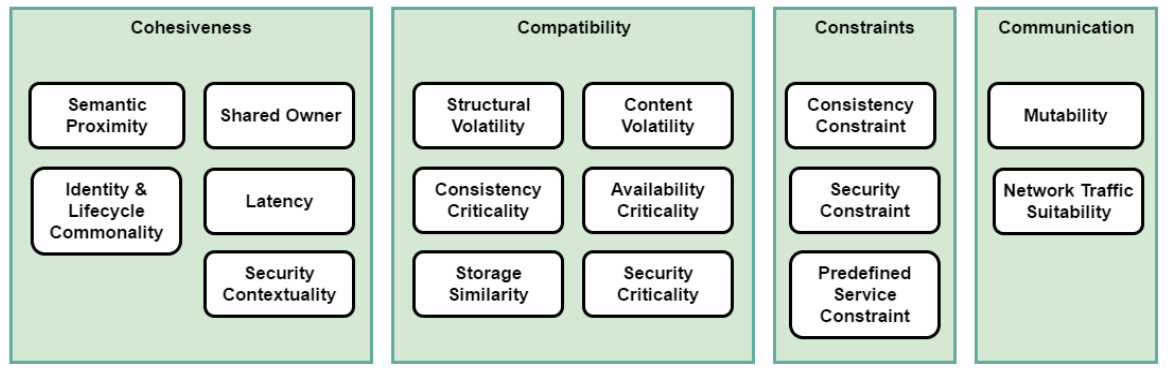
\includegraphics[width=\textwidth]{img/service_cutter_16_criteria.png}
     	\end{center}
     	\caption{Critérios de acoplamento propostos por \cite{gysel16_service_cutter}}
     	\floatfoot{Source: \cite{gysel16_service_cutter}}
     	\label{fig:service_cutter_16}
 	\end{figure}
   
   Esta técnica suporta atualmente duas técnicas de \textit{clustering}: \textit{Epidemic Label Propagation} por \cite{leung2009TowardsRC} e o algoritmo de \cite{girvan01_community_structure_cluster}.
   
   No entanto, o \textit{Service Cutter} não tem capacidades de extrair a informação basal necessária para o seu funcionamento de um projeto de \textit{software}, estando altamente dependente dos artefactos de \textit{software} disponibilizados pelo utilizador. Este facto poderá ser limitante em vários sentidos. Em primeiro lugar por se considerar que a documentação é considerada muitas vezes como escassa e desatualizada, em especial nas metodologias atuais Ágeis, que se assentam maioritariamente no \textit{feedback} do utilizador e não em desenvolvimento de documentação. Em segundo lugar, pela necessidade de haver uma correspondência entre os artefactos produzidos e os artefactos esperados pelo \textit{Service Cutter}. 
    
    % o service cutter apenas aceita .json, quão fácil será a conversão de UML para json?
   
    % Service Cutter

    % From Monolith to Microservices: A Dataflow-Driven Approach
    % https://ieeexplore.ieee.org/document/8305969
    
    \cite{chen17_dataflow_driven} seguiram também uma abordagem orientada aos modelos recorrendo a \textit{data-flow diagrams (DFD)}. A sua abordagem é descrita em três fases: é realizada uma análise de requisitos de negócio por parte dos engenheiros juntamente com os utilizadores, para a obtenção do \textit{data-flow diagram}; de seguida, o seu algoritmo combina o diagrama recolhido com as mesmas operações num diagrama abstracto virtual; e por último recorre a este diagrama virtual para extrair propostas de micro-serviços. \cite{chen17_dataflow_driven} fazem de seguida uma comparação com o \textit{Service Cutter} dada alguma semelhança na abordagem por modelos de ambos os trabalhos, argumentando que o seu é mais fácil de operar, por recorrer a diagramas mais simples de construir; mais racional e objetivo, por não realizar decomposições desnecessárias deixando entidades que fazem sentido estar juntas em serviços diferentes; e mais fácil de entender por apresentarem os serviços extraídos de uma forma mais intuitiva. Esta comparação foi no entanto realizada para casos de estudo bastante limitados podendo potenciar as características de uma ferramenta relativa a outra.
    
    Embora todas estas melhorias apresentadas relativas ao \textit{Service Cutter} esta abordagem a modelos encontra-se limitada por alguns pontos cruciais. Em primeiro lugar, a combinação feita entre os modelos e as operações é realizada baseada nos nomes das operações, obrigando a que o DFD siga de forma restrita a convenção de nomes utilizado nas operações de CRUD \citep{chen17_dataflow_driven}. Em segundo lugar, este processo realiza maioritariamente a proposta de serviços recorrendo às operações de dados realizadas na lógica de negócio, no entanto, caso haja a necessidade de lidar com outras capacidades que não estejam estritamente ligadas aos dados e suas operações, as propostas de serviços serão de uma granularidade mais elevada. Por último, a comparação feita com o \textit{Service Cutter} recorrendo a casos de teste bastante simples limita a validação relativamente à capacidade de lidar com a extração de serviços em aplicações de larga escala.
    
    Analogamente ao \textit{Service Cutter} a proposta de \textit{DFD} é também altamente dependente da qualidade dos artefactos proporcionados pelo seu utilizador. Os artefactos poderão necessitar de conversão para os devidos formatos suportados pelas ferramentas; processo que não é automatizado e pode resultar na degradação da qualidade dos artefactos.

    % perde-se muita informação por se trabalhar com diagramas de alto nivel     
    % tem sempre o problema de ser input heavy para o utilizador
    
    % operações: extract, query, compose, integrate?
    % operações: crawl, extract, parse

\newpage
\section{Sumário}

    Com base na investigação e análise da bibliografia referida nas secções anteriores, realiza-se agora uma discussão acerca das abordagens apresentadas: migração orientada a código fonte estática, migração orientada a código fonte dinâmica e migração orientada a modelos.
    
    Começando pela última, migração orientada a modelos, \cite{gysel16_service_cutter} e \cite{chen17_dataflow_driven} apresentam duas abordagens promissoras pelas técnicas que abordam no entanto muito limitadas pelo facto de estarem altamente dependentes do \textit{input} do utilizador. Esse \textit{input} de artefactos deve seguir regras específicas e estar de acordo com os formatos e regras impostas pelo \textit{software}. Este processo de pré-processamento do \textit{input} e conversão para ir de encontro às regras estabelecidas pode ser por si só um trabalho moroso e que necessite de um investimento de tempo elevado.

    
    As soluções orientadas ao código fonte segundo uma abordagem dinâmica permitem a obtenção de informação extra que abordagens estáticas não permitem. \cite{fome_jin_18} recorrem aos \textit{logs} de execução para segundo eles fazerem uma identificação de funcionalidade mais confiável. Este tipo de abordagens está no entanto limitado por dois factores: o primeiro apresenta-se sobre a carga extra colocada sobre o sistema para a recolha de \textit{logs} durante a execução, podendo ser um problema em sistemas de larga escala; em segundo, pela forma como esta recolha está limitada pelos casos de teste realizados para execução e recolha dos respetivos \textit{logs}. A criação de testes de forma incompleta e com um \textit{coverage} inadequado resultará também em proposta de micro-serviços inadequadas. A geração de testes que retratem o comportamento do utilizador de forma automatizada é também uma tarefa complexa, para a qual ainda não existem soluções concretas.
    
    Por último surgem as abordagens baseadas na manipulação de código fonte de forma estática. Destacam-se logo à partida por serem abordagens que recorrem estritamente ao código fonte, não existindo a necessidade de outros artefactos ou um elevado investimento de pré-processamento para a aplicação da respetiva técnica por parte do utilizador final. Comparativamente com as abordagens dinâmicas, não necessitam de qualquer tipo de execução do código ou \textit{logging} o que as torna mais promissoras para análise de aplicações de grande escala.
    
    Neste tipo de abordagens estáticas, e considerando os trabalhos que para além da realização de propostas de micro-serviços, também realizam a extração para os respetivos serviços, o principal ponto identificado como falha é a granularidade de \textit{refactoring} das propostas. A extração é feita sempre recorrendo a classes como o nível atómico o que limita os processos de \textit{refactoring} das novas propostas de micro-serviços.
    
    % talvez explicar porque é que limita?
    
    
% sistema que não necessita de um input elevado por parte do utlizador (já existem alguns assim, mas é uma mais valia)
% ServiceCutter

% NOTAS: Towards a Framework for generating program source dependence graphs from source code

% Ferramentas como o OPAL, Soot e WALA recorrem a código compilado para a construçao do \textit{program dependence graph}.

% Atlas constrói o grafo apartir de \textit{source code}, mas dada a sua integração com o \textit{Eclipse} é necessário que o código seja compilado e todas as suas dependências estejam resolvidas.  

% Dado o \textit{source code} de um programa, em primeiro lugar ele é convertido para uma gramática que o interpretador por eles proposto perceba.


